\subsubsection{本走行・実験走行で見つかった課題}
\paragraph{走行不可能領域への侵入でロボットが動作不能になる問題}
むぎまるチームは本走行において, 横断歩道の途中で
navigation2がナビゲーションを中断し, 
動作不能に陥ったことでリタイアとなった. 
この原因は, navigation2が経路生成時に参照するコストマップにおいて, 
ロボットが走行できない領域(以降「走行不可能領域」)に侵入したことであった. 
%↑@@@文分けましょう. あるいは図を見せる前から細かすぎるのでもっと要約する. 
この状況をRvizを用いて可視化した際の画像を図\ref{fig:mugimaru_result}に示す. 
図中のピンク色の範囲は走行不可能領域のコスト, 
水色の範囲はロボットの内接円半径を考慮した走行不可能領域のコストを表している. 
つまり, ロボットの中心が水色の範囲に侵入すると
ロボットが走行不可能領域にいると判断される. 
%%%中心の話をするなら画像内でも中心を表現したほうが見やすい気がする. 
%%%↑図に中心の表現を追加
図\ref{fig:mugimaru_result}からロボットの中心は
水色の範囲に侵入していることが確認できる. 
この状態になった後, プランナーから
%@@@これは使うプランナーによる@@@
経路及び動作の生成が実施されなかった. 
その後, リカバリー動作が実行されたが, 
有効に働かずナビゲーションを中断してしまった. 

この問題への対策としては, 
グローバルプランナーで経路を算出する方法ではなく, 
文献\cite{ueda2023JRM}で用いられている価値反復のように, 
ロボットが存在しうる位置, 向きすべてに対して行動を
割り付ける方法(最適方策を求める方法)を導入することが考えられる. 
価値反復の場合は, 走行に適さない位置に
(無限大ではない)大きなペナルティーを与えておき, 
その領域で行動計画をすると, 
そこから脱出する行動が割り付けられるので, 
動作が中断されることはない. 


%この問題への対策として, 走行可能領域に入るまで
%障害物を回避しながら動き回るという復帰動作を実装することが
%一つ挙げられる. 
%図からロボットの前方には走行可能領域があることが確認できる. 
%その場所までLiDARにより周囲の障害物を検知して, 
%それらを回避しながら移動可能であれば, 
%この問題が発生した場合にでもナビゲーションを続行できるようになると考える. 


\begin{figure}[h]
  \begin{center}
  	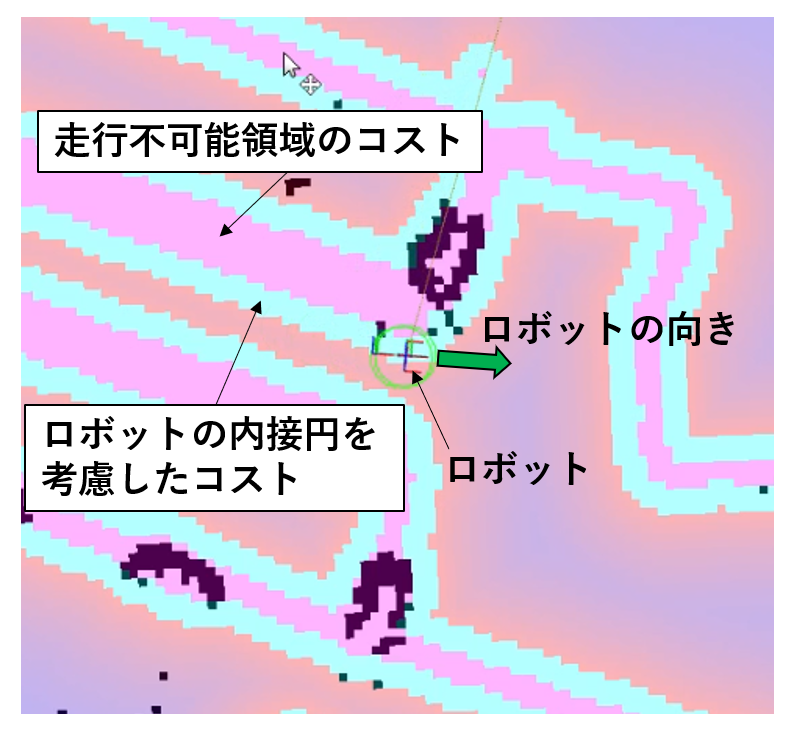
\includegraphics[width=0.9\linewidth]{figs/mugimaru_result.eps}
  	\caption{ロボットがコストマップに乗り上げた状況の図} 
  	\label{fig:mugimaru_result}
  \end{center}
\end{figure}

